\documentclass{sig-alternate-10pt}
\usepackage{pgf}
\usepackage{tikz}
\usepackage{verbatim}
\usepackage{url}
\usepackage{hyperref}	% Clickable links to figures, references and urls.
\usepackage{basicobjpgftikz}	% Custom basic shapes using pgf/tikz.
%\usepackage{Sig-alternate-10pt}
%\setlength{\oddsidemargin}{0in}
%\setlength{\evensidemargin}{0in}
%\setlength{\headheight}{12pt}
%\setlength{\headsep}{60pt}
%\setlength{\topmargin}{-90pt}
%\setlength{\textwidth}{6.5in}
%\setlength{\textheight}{10in}

\begin{document}

\title{Access Control in Amoeba}
\author{Attique Dawood}
\maketitle

\section{Introduction to Amoeba}

Amoeba is a distributed operating system developed at Vrije Universiteit, Amsterdam, in the eighties. Chief designer was Andrew S. Tanenbaum. The architecture can be described as a composition of workstations, terminals, processor pool and servers connected through LAN (figure~\ref{amoeba-architecture}). Servers are responsible for file management, printers, login authentication and database etc.

It was designed to be transparent with user not having to worry about underlying hardware, like number of processors. The user only sees interacting with a single powerful system~\cite{amoeba-sourceforge}. Another important design goal was to have an \emph{object-based} resource management~\cite{distributed-systems-coulouris} where each resource is regarded as an object.

\begin{figure*}[here, trim axis left]
\centering
\begin{tikzpicture}

	\draw[line width=1.5pt] (3,0) -- (0.6,4);
	\draw[line width=1.5pt] (3,0) -- (2.6,4);
	\draw[line width=1.5pt] (3,0) -- (4.6,4);
	\Xterminal{0}{4}{1}{1}{0}{0}
	\Xterminal{2}{4}{1}{1}{0}{0}
	\Xterminal{4}{4}{1}{1}{0}{0}
	\coordinate [label=above: \textsf{X terminals}] (XTerminals) at (2.6,5.5);
	
	\draw[line width=1.5pt] (3,0) -- (8.6,1.6);
	\draw[line width=1.5pt] (3,0) -- (8.6,-0.5);
	\Workstation{8}{-1}{1}{1}{0}{0}
	\Workstation{8}{1}{1}{1}{0}{0}
	\coordinate [label=above: \textsf{Workstations}] (Workstations) at (8.6,-2);
	
	\draw[line width=1.5pt] (3,0) -- (0.6,-2);
	\draw[line width=1.5pt] (3,0) -- (2.1,-2);
	\FileServer{0}{-3}{1}{1}{0}{0}
	\FileServer{1.5}{-3}{1}{1}{0}{0}
	\coordinate [label=below: \textsf{File servers}] (FileServers) at (1,-3.5);
	
	\draw[line width=1.5pt] (-2.75,-2.5) -- (-4,-2.5);
	\coordinate [label=left: \textsf{WAN}] (WAN) at (-4,-2.5);
	
	\draw[line width=1.5pt] (3,0) -- (-2.5,-2.5);
	\Server{-3}{-3}{1}{1}{0}{0}
	\coordinate [label=below: \textsf{Gateway}] (Gateway) at (-2.7,-3.5);
	
	\draw[line width=1.5pt] (3,0) -- (3.8,-2);
	\draw[line width=1.5pt] (3,0) -- (4.8,-2);
	\draw[line width=1.5pt] (3,0) -- (5.8,-2);
	\Server{3.5}{-3}{1}{1}{0}{0}
	\Server{4.5}{-3}{1}{1}{0}{0}
	\Server{5.5}{-3}{1}{1}{0}{0}
	\coordinate [label=below: \textsf{Login, print and other servers}] (Servers) at (5,-3.5);
	
	\draw[line width=1.5pt] (3,0) -- (-4.8,2);
	\ProcessorPool{-5}{0}{1}{1}{0}{0}
	\coordinate [label=below: \textsf{Processor pool}] (ProcessorPool) at (-3.85,-0.5);
	
	\TextCloud{3}{1}{2}{2}{0}{0}{\textsf{\begin{large}Local Area Network\end{large}}}

\end{tikzpicture}
\caption{Amoeba architecture.}
\label{amoeba-architecture}
\end{figure*}

\section{Objects and Capabilities}

\emph{Object-oriented} design is a relatively new concept in computing. The \emph{capability-based} systems support object-oriented computing. Following sections give a brief description of objects and capabilities in Amoeba.

\subsection{Objects}

An \emph{object} is described by its \emph{data members} and \emph{operations}. In amoeba every resource is treated as an object. An object can be any physical or logical entity. Examples of objects are files, memory segment, processes, terminals, message port, I/O devices etc. Objects are assigned \emph{identifiers} by a naming server.

\subsection{Capabilities}

All objects are described and protected by \emph{capabilities}. A capability is a token, key or ticket which provides access to a resource or object. Unlike conventional systems, capabilities provide \emph{``a single mechanism to address both primary and secondary memories and a single mechanism to address both software and hardware resources.''}~\cite[p.~3]{capability-based-systems-levy}

\section{Capabilities and Access Control}

Capabilities are implemented as a data structure having at least two fields, the \emph{object identifier} and \emph{access rights}. In Amoeba, a capability is a 128 bit data structure with four fields as shown in figure~\ref{capability-DS}.

\begin{figure*}[here, trim axis left]
\vspace{0.5cm}
\centering
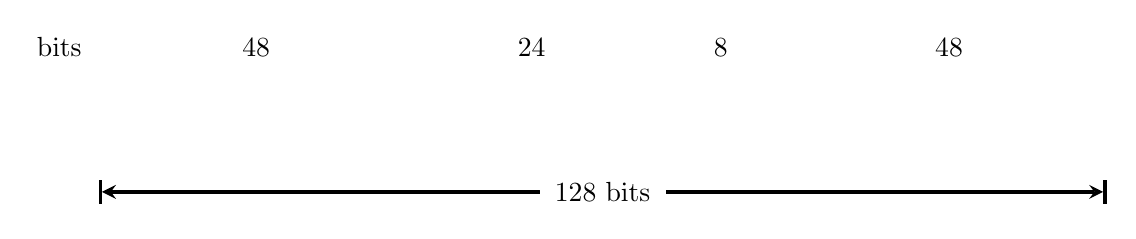
\begin{tikzpicture}

	\CapabilityDS{0}{0}{1}{1}
		{\textsf{\begin{footnotesize}Server port\end{footnotesize}}}
		{\textsf{\begin{footnotesize}Object ID\end{footnotesize}}}
		{\textsf{\begin{footnotesize}Permissions\end{footnotesize}}}
		{\textsf{\begin{footnotesize}Check field\end{footnotesize}}}
	
	\coordinate [label=above:bits] (bits) at (-0.5,1.2);
	\coordinate [label=above:48] (48Bits) at (2.0,1.2);
	\coordinate [label=above:24] (24Bits) at (5.5,1.2);
	\coordinate [label=above:8] (8Bits) at (7.9,1.2);
	\coordinate [label=above:48] (48Bits) at (10.8,1.2);
		
	\draw[very thick, >=stealth, |<->|] (0,-0.4) -- (12.8,-0.4);
	\draw[white,very thick] (5.6,-0.4) -- (7.2, -0.4);
	\coordinate [label=below:128 bits] (128bits) at (6.4,-0.15);

\end{tikzpicture}
\caption{Fields in the capability data structure.}
\label{capability-DS}
\end{figure*}

\subsection{Capability Fields}

The \emph{server port} field identifies the server on which the object is located. A unique identifier \emph{object ID} is used to locate the requested object such as a file or memory segment. The \emph{permissions} field lists all the operations that can be performed on the object. For example, a user has capability for a file with read--only permissions. That file can only be read by the user in question.

Users, processes or procedures, generally referred as \emph{subjects}, possess a \emph{list of capabilities}. This list defines their rights and permissions for accessing resources available to them. It is important to note that capabilities list exists in \emph{user space}. There is a need to protect against forgery. This is accomplished with the \emph{check field} which is a 48 bit random number. This is used together with the permissions field to provide integrity checks against any tampering.

\subsection{\texttt{filewrite} Example}

A user (or process) cannot access an object unless it has the capability for that object in its capability list with suitable permissions. To specify an object, it would provide the \emph{index} for that capability from its list~\cite[p.~4]{capability-based-systems-levy}. To write a string ``message'' onto a file he can use a \emph{filesystem} function as,
\begin{verbatim}
filewrite (file_capability, "string");
\end{verbatim}
The \texttt{file\_capability} provides the name of the file user is trying to access and whether he has \emph{write} permissions. The \emph{fileserver} (where the file resides) would check against the capability provided by the user with its database and allow/disallow access.

\subsection{Reduced Capabilities}

When a user creates an object (or resource) on a server, it is provided \emph{owner} capability with all the permission bits set. The user can do anything with that particular object including deleting it altogether. Users with owner permissions often want to give reduced access to others~\cite[ch.~2]{distributed-systems-coulouris}, e.g. read--only access to a file.

Amoeba provides a one--way function $f$ to compute reduced capability $r'$ from owner's capability check field $c$. Reduced capability check field is generated by taking $exclusive-OR$ of $r'$ and $c$ and using the result as input to $f$ (figure~\ref{reduced-capability}). The resulting reduced capability check field can be expressed as $f(r'~XOR~c)$.

\begin{figure}[here, trim axis left]
\vspace{-0.2cm}
\centering
% Figure scaled down 50 %.
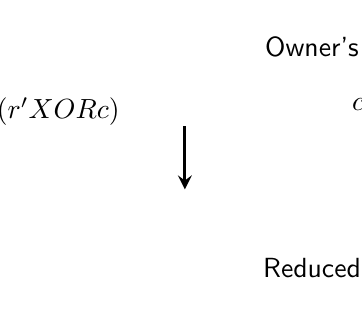
\begin{tikzpicture}

	\CapabilityDSScaled{0}{0}{0.5}{0.5}{$s$}{$o$}{$r$}{}
	\coordinate [label=below:\textsf{$c$}] (Permissions) at (5.4,0.375);	
		
	\draw[very thick, >=stealth, ->] (3.2, -0.1) -- (3.2, -0.9);
	\CapabilityDSScaled{0}{-1.5}{0.5}{0.5}{$s$}{$o$}{$r'$}{$f(r'~XOR~c)$}
	
	\coordinate [label=above:\textsf{Owner's capability}] (Owner) at (3.2,0.6);
	\coordinate [label=below:\textsf{Reduced capability}] (Reduced) at (3.2,-1.65);
	
\end{tikzpicture}
\caption{Deriving reduced capability from owner's capability.}
\label{reduced-capability}
\end{figure}

\section{Capabilities and Access Control List (ACL)}
Capabilities--based systems provide object--oriented abstraction and this approach can be applied to many computer design problems. Object--oriented implementation has the inherent advantages of uniformity, data abstraction and information hiding. Maintainability is also much easier as system becomes more sophisticated and size grows. ACLs require authentication at each access compared to capabilities where only one--time authentication is required.

Despite the advantages there are also disadvantages of capabilities. Capabilities cannot prevent man--in--the--middle attacks like eavesdropping and replaying. Compared to ACLs, capabilities cannot be easily retracted~\cite{distributed-systems-coulouris}. If Alice and Bob have capabilities to access a resource and the owner wants to restrict Bob's access, a new set of capabilities must be issued invalidating the old capabilities. Alice also needs to be issued the new capability. Also, since capabilities work as keys, Alice can simply give her new capability to Bob and allow access against owner's consent.

\nocite{*}
\bibliographystyle{ieeetr} %plain, ieeetr
\bibliography{Amoebaref}

\end{document}




